\pdfoutput=1
\documentclass[cits]{JINST}
\newcommand{\unit}[1]{\ensuremath{\mathrm{\,#1}}}
\renewcommand{\u}[1]{\unit{#1}}
\newcommand{\um}{\textmu m}
\DeclareFontFamily{U}{euc}{}
\DeclareFontShape{U}{euc}{m}{n}{<-6>eurm5<6-8>eurm7<8->eurm10}{}
\DeclareSymbolFont{AMSc}{U}{euc}{m}{n}
\DeclareMathSymbol{\umu}{\mathord}{AMSc}{"16}
\usepackage[justification=centering]{caption}
\usepackage[pdftex]{graphicx}
\usepackage{amsmath}
\usepackage{afterpage}
\usepackage{wrapfig}
\usepackage{tabularx}
\usepackage{subfigure}
\usepackage{caption}
\usepackage{tabu}
\usepackage{booktabs}
\usepackage{multicol}
\newcommand{\comment}[1]{{\fontsize{10}{10}{\par \tt\textbf {\selectfont #1}} \par}}

\graphicspath{{figs/}}

\title{Close-by showers separation within SDHCAL prototype detector using ArborPFA}

\author{R. \'Et\'e$^a$\thanks{Corresponding author.} \\%, I. Laktineh$^a$ , G. Grenier$^a$ , A. Steen$^a$ , L. Mirabito$^a$\\
\llap{$^a$} Universit\'e de Lyon, Universit\'e Lyon 1, CNRS/IN2P3, 
 IPNL, 4 Rue E.~Fermi, 69622 Villeurbanne Cedex, France\\
 
 
 E-mail: \email{rete@ipnl.in2p3.fr}
 }
 
\abstract{ After the validation of the PandoraPFA algorithm, a new reconstruction algorithm is needed in order to validate the Particle Flow Algorithm (PFA) approach. In a such designed detector, the electromagnetic calorimeters (ECAL) and hadronic calorimeters (HCAL) have a leading role in the reconstruction task. The Semi-Digital Hadron Calorimeter (SDHCAL) is a candidate prototype of hadron calorimeter for ILD since its fine granularity allows to apply the Particle Flow Algorithm. The ArborPFA algorithm has been applied to the SDHCAL detector prototype data \cite{sdhcal-paper} in order to extract the single particle algorithm efficiency and to separate close-by hadronic shower contributions. The results of these studies indicate a good single particle efficiency and powerful separation up to 5 cm of separation distance.}

\begin{document}

\keywords{Keywords: Particle flow; Calorimetry; ILC; SDHCAL}

\section{Introduction}
%%%%%%%%%%%%%%%%%%%%%%%%%%%%%%%%%%%%%%%%%%%
%%%%%%%%%%%%%%%%%%%%%%%%%%%%%%%%%%%%%%%%%%%

~~~~~~~After the Higgs boson discovery at LHC, a linear e$^+$ e$^-$ collider such as the ILC is foreseen in order to measure precisely its properties. An important requirement of such a machine should be a good jet energy resolution ($\Delta$E/E $\sim$3-4\%) and thus the ability to distinguish Z, W$^{\pm}$ and Higgs bosons. Since the hadronic branching fractions of these bosons is expected to be dominant, a good energy resolution and a fine transverse segmentation both must be provided by the \textit{electromagnetic calorimeter} (ECAL) and the \textit{hadronic calorimeter} (HCAL).

The calorimeters proposed by the CALICE collaboration are currently under study mainly for this purpose. A \textit{semi digital hadronic calorimeter} prototype (SDHCAL) has been constructed \cite{sdhcal-paper} and successfully tested at the CERN H2 and H6 test beam lines of the SPS (CERN) in May and August 2012 respectively. With a transverse readout segmentation of 1 cm$^2$, 48 GRPC layers of $\sim$ 2.7 cm (absorber+active medium) and a good energy resolution ($\frac{\sigma_{E}}{E}$ $\simeq$ 10 \%), this calorimeter fits perfectly the ILC needs. 

On the other hand, the Particle Flow concept has been introduced in order to achieve the ILC benchmarks \cite{ilc-tdr}. This algorithm aims to reconstruct particles individually using the most appropriate detector for the energy and momentum measurement. An implementation of the particle flow algorithm called PandoraPFA has been developed by M. A. Thomson \cite{pandora-pfa} and is the most mature implementation of this algorithm for linear colliders.

In this paper, we would like to present an other approach of the particle flow : the ArborPFA approach. The algorithm has been designed for high granularity calorimeters and tested on SDHCAL test beam data. First, we evaluate here the performance of the algorithm on single pion particles. Then, we present the result of a study that aims to separate two overlaid pion showers with different separation distances and different energies.

\section{The SDHCAL prototype}

The SDHCAL prototype is a sampling calorimeter which consists in 48 layers alternating a 20 mm steel absorber slice and a 7 mm gas resistive plate chamber (GRPC) slice. The gas gap between the two electrodes of the GRPC is 1.2 mm. 9216 pads (96 x 96) of 1cm$^2$ compose the readout of each chamber, thus the total number of channels  comes to 442368. A complete description of the calorimeter setup and its features can be found in \cite{sdhcal-paper}. 

The test beam data used in this paper have been taken at the CERN H6 beam line of the SPS in August/September 2012. The pion event selection is also done according to \cite{sdhcal-paper}.

The reconstructed energy is computed as follows :

\begin{equation}
  E_{rec} = \alpha(N_{hit}).N_{1}
          + \beta(N_{hit}) .N_{2}
          + \gamma(N_{hit}).N_{3}   
\end{equation}
where $\alpha$, $\beta$ and $\gamma$ are quadratic functions of the number of hits N$_{hit}$ and N$_1$, N$_2$ and N$_3$ are the number hits of threshold 1, 2 and 3. The nine parameters of these functions are extracted from a $\chi^2$ minimization :

\begin{equation}
  \chi^2 = \sum\limits_{evt} \frac{(E_{beam} - E_{rec})^2}{E_{beam}^2}
\end{equation}
over the energy range [10, 80] GeV by step of 10 GeV. The final parameters and the three function shapes are summarized in the figure \ref{SDHCAL_CALIBRATION} in annexe of this document. The linearity and energy resolution will be shown in the section \ref{SINGLE_PARTICLE_STUDY_SECTION} dedicated to the single particle study.

\section{The Arbor particle flow algorithm}
%%%%%%%%%%%%%%%%%%%%%%%%%%%%%%%%%%%%%%%%%%%
%%%%%%%%%%%%%%%%%%%%%%%%%%%%%%%%%%%%%%%%%%%

\subsection{Principle} 
%%%%%%%%%%%%%%%%%%%%%%%%%%%%%%%%%%%%%%%%%%%

~~~~~~~The Arbor approach has been developed by H.Videau in the ALEPH experiment at LEP and adapted by M.Ruan \cite{arbor-manqi} for ILD detector design. It is based on the idea that the shower reconstruction looks like the shower structure itself : a tree topology. 

The figure \ref{ARBOR_STRUCTURE} shows the shower development after a proton interaction (left) for which we can see the multiple components of the shower : charged particles, neutral particles, electromagnetic and hadronic parts. 
In the calorimeter view, we can see the shower tree after ArborPFA reconstruction which shows also the analogy between vertexes versus calorimeter hits and particle trajectories versus connector links.

With such an approach, the shower reconstruction follows a principle close to the underlying physics and can be useful for studying the shower structure. Such studies have already been done by comparing the track length of Monte-Carlo particles produced within a shower and branch lengths in reconstructed Arbor trees \cite{arbor-manqi}.
  
\begin{figure}[!ht]
  \begin{center}
    
\includegraphics[width=0.45\linewidth]{ProtonDecay.png} \hfill
    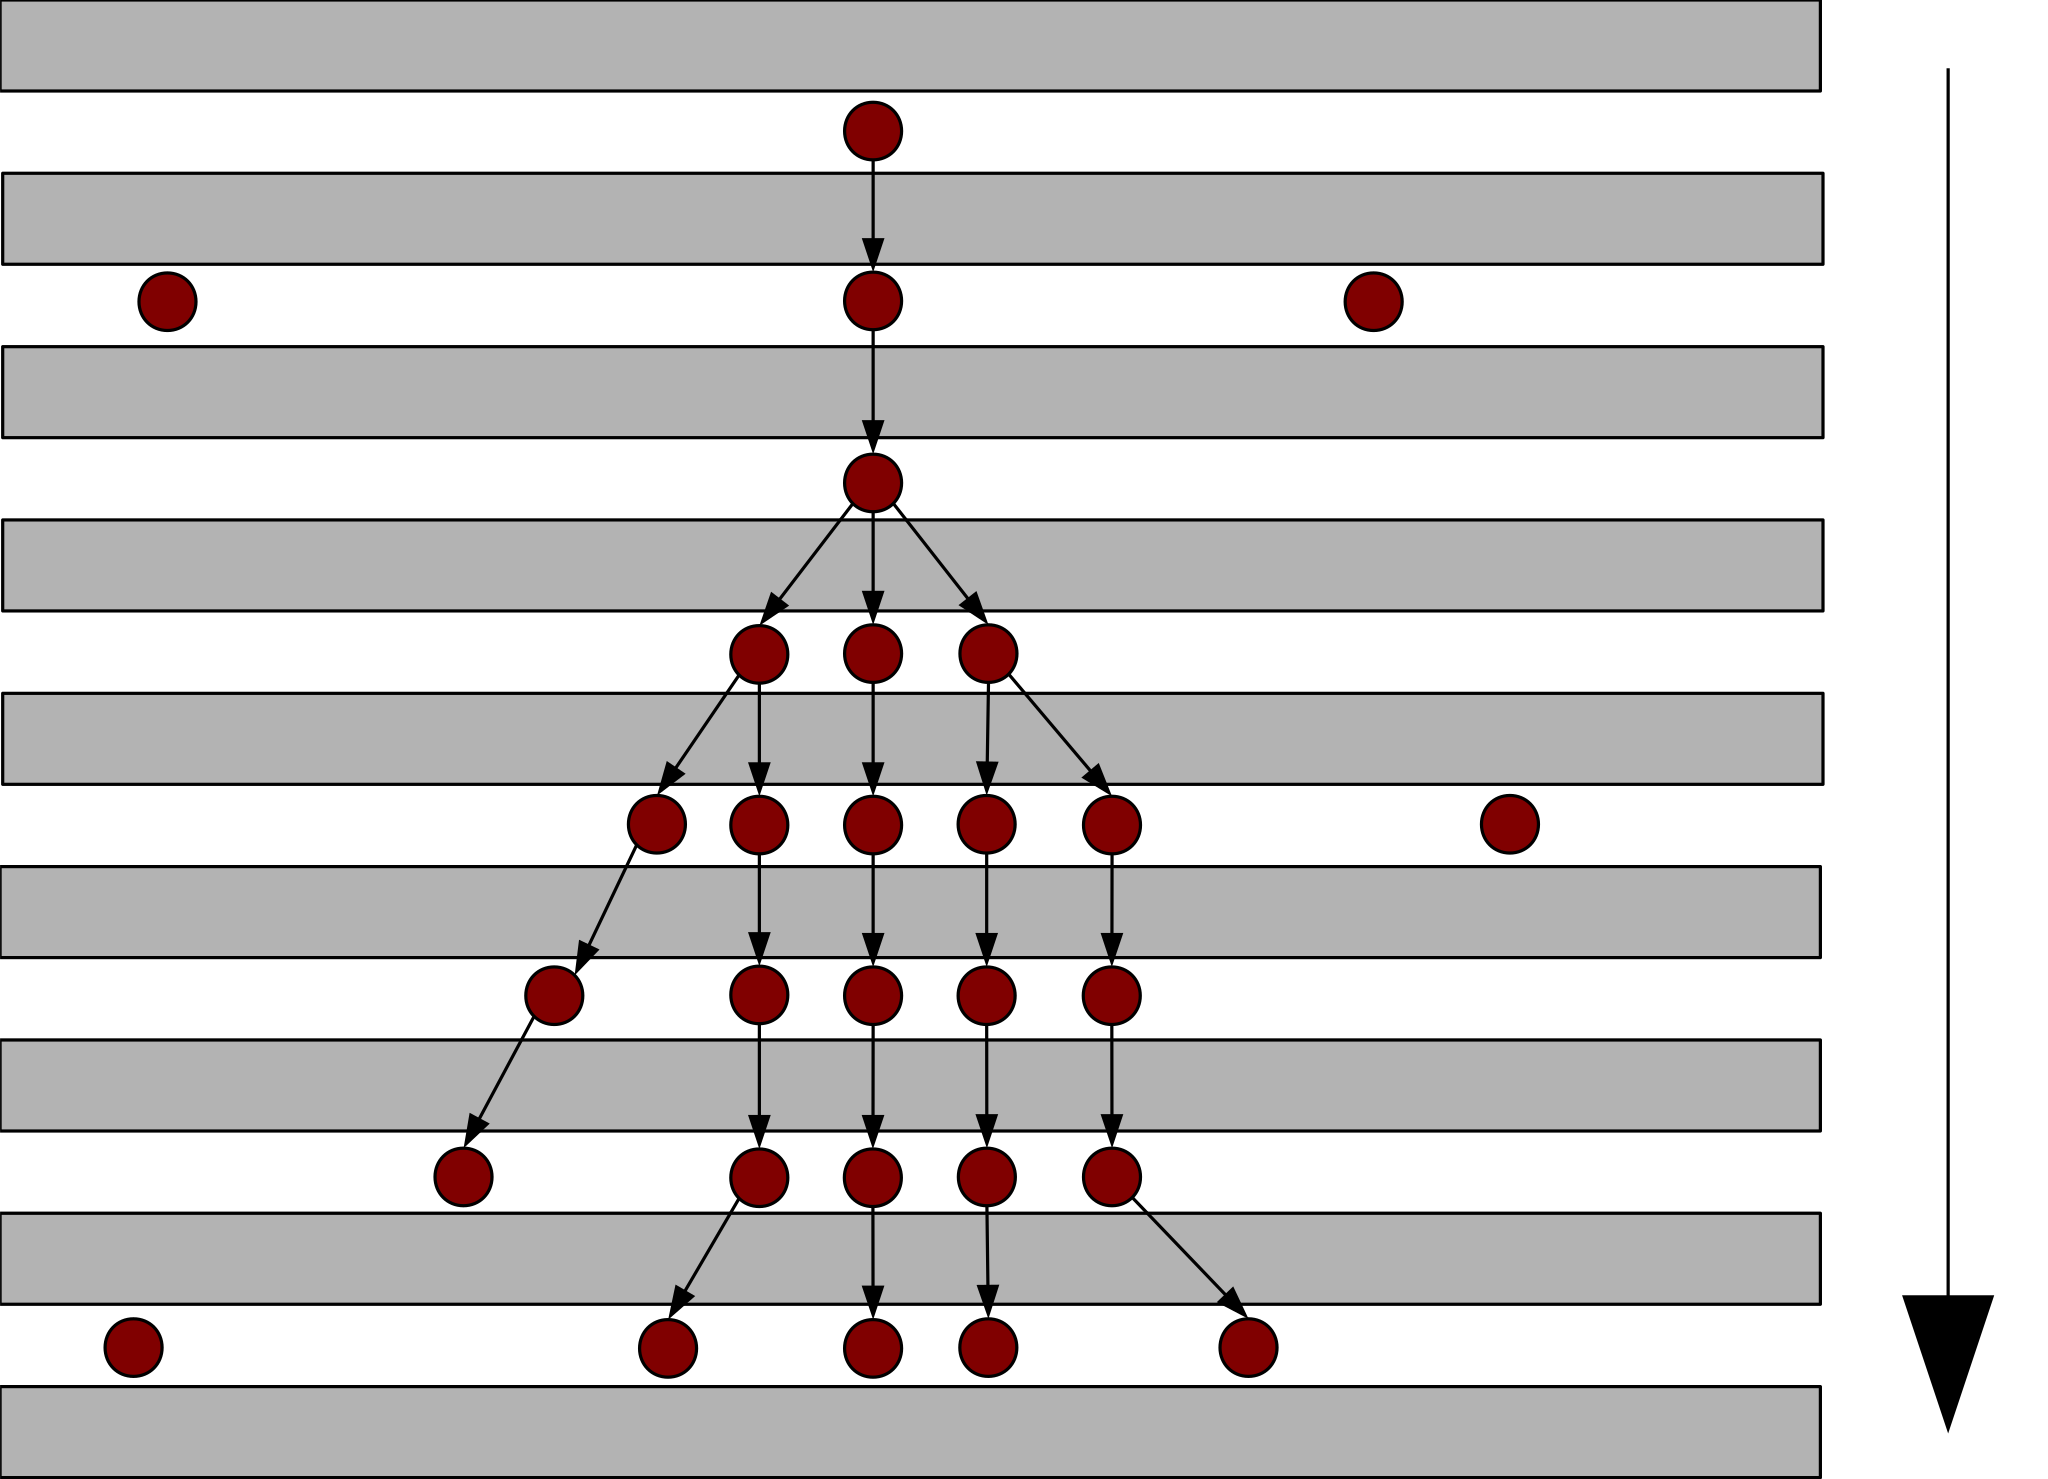
\includegraphics[width=0.45\linewidth]{ArborSchema.png}
  \end{center}
  \caption{\label{ARBOR_STRUCTURE} Left : schematic view of an induced proton shower. Right : schematic view of a reconstructed shower in a calorimeter with calorimeter hits (in red) and connectors (in black) clustered in an oriented tree topology by ArborPFA}
\end{figure}

This version of the algorithm is implemented using the PandoraSDK API as a toolkit for generic PFA development. The API is used in a Marlin c++ processor as part of the reconstruction chain in ILCSOFT \cite{ilcsoft}. It produces only a ROOT \cite{root} file containing the variable needed for the analysis described in this document.

Before describing the algorithm contents in detail, we would like to introduce some definitions specific to ArborPFA.

\paragraph*{Object} An \textit{object} is a calorimeter hit or a group of contiguous calorimeter hits within a layer that serves as vertex for the ArborPFA algorithm. This was introduced for two reasons i) provide a generalization of connections between \textit{objects} without making any assumptions of what is contained in an \textit{object}, ii) fight against the multiplicity in gaseous based calorimeters such as SDHCAL \cite{sdhcal-paper}.

\paragraph*{Flow direction} The flow direction is of two types : forward direction which is from an inward layer to a forward layer and backward direction for the opposite.

\paragraph*{Connector} A connector is a link between two \textit{objects}. It has a weight and a direction.

\paragraph*{Connector depth} The connector depth is defined as the number of connector needed to reach an object starting from an given one. For example, for a given object, one of the forward connectors has a depth of one. A forward connector of a forward connector of this object has a depth of 2.

\paragraph*{Tree} A tree is a set of \textit{objects} connected in a tree topology which means that for each object there is only one backward connector. An \textit{object} without backward connector is called a seed and an \textit{object} without forward connector is called a leaf.

\paragraph*{Cluster} A cluster is a set of trees and isolated \textit{objects} which are not connected with any other \textit{object}.

\paragraph*{Particle flow object (PFO)} A particle flow object is a set of clusters and tracks which corresponds to a reconstructed particle.

\subsection{Pre-clustering phase} 
%%%%%%%%%%%%%%%%%%%%%%%%%%%%%%%%%%%%%%%%%%%

~~~~~~~Before building trees, we need to create objects to connect with each others. Once objects are created, an additional algorithm is run in order to identify isolated objects that are not part of a shower bulb. These objects will be treated in special way in the main clustering algorithm.

%%% OBJECT CREATION %%%
\begin{wrapfigure}{r}{0.4\textwidth}
  \vspace{-20pt}
  \begin{center}
    \includegraphics[width=\linewidth]{ObjectCreationAfter.pdf}
  \end{center}
  \vspace{-10pt}
  \caption{\label{ARBOR_OBJECT_CREATION} Schematic view of the object creation output. Small groups of contiguous calorimeter hits are group together (encircled).}
  \vspace{-20pt}
\end{wrapfigure}

\paragraph*{Object creation} When a minimum ionizing particle (MIP) goes through the detector, many pads can be fired in a single layer and leads to a multiplicity greater than 1. To overcome the problem, intra-layer clusters are built. For each cluster, if its number of calorimeter hits is greater than 4, the cluster is split up and each calorimeter hit becomes an object. This happens generally in the main part of a shower. In the other case, an object is created and can contains from 1 up to 4 calorimeter hits. This is the case for MIPs or isolated group of hits. 

%%% MIP TAGGING %%%
\paragraph*{Mip track candidate tagging}
Due to inefficiencies of MIPs (minimum ionising particles) crossing the sensitive zone and in order to retrieve correctly the primary track in the calorimeter, MIPs hits, so in our case MIPs \textit{objects}, are identified and tagged for a future treatment. The tagging is performed with respect to other objects proximity within a layer and in different layers around the object of interest.

\subsection{The main clustering phase - Connectors and trees}
%%%%%%%%%%%%%%%%%%%%%%%%%%%%%%%%%%%%%%%%%%%

~~~~~~~The main clustering algorithm can be decomposed in sub-algorithms :
\begin{itemize}
  \item The connector loop, where a loop over algorithms is performed in order to create and remove connectors. At the end of this step, all the objects are arranged in a tree structure which means that each object has 0 or 1 connector in the backward direction and 0 or meanies in the forward one.
  \item The tree clustering, which create clusters containing each a tree structure left by the previous algorithms.
\end{itemize}

In the current implementation, the connector loop contains the following algorithms :

\begin{wrapfigure}{r}{0.45\textwidth}
  %\vspace{-15pt}
  \begin{center}
    \includegraphics[width=\linewidth]{ConnectorSeeding1.pdf}
  \end{center}
  \vspace{10pt}
  \caption{\label{ARBOR_CONNECTOR_SEEDING_1} Schematic view of a neutral and a charged pion showers after the first connector seeding algorithm}
  %\vspace{-15pt}
\end{wrapfigure}

\paragraph*{Primary track connection} This algorithm aims to create connections between objects belonging to the primary track of charged particles in the calorimeter. It consists mainly in creating a sub object list that are candidates for the primary tracks by using the previously tagged objects (see Mip track candidate tagging algorithm) and by using the track extrapolations on the calorimeter front face. Once this list is built, the connector seeding 1 algorithm and the connector cleaning 1 are run on the sub list only. These two algorithms are described below in details.

\paragraph*{Connector seeding 1} In this sub-part, we start by creating a lot of connections in the neighbourhood of each object. For each object, we look for other objects in the N$_{layers}$ next layers with a maximum distance $\Delta_{max}$ and we create a connection between them. The figure \ref{ARBOR_CONNECTOR_SEEDING_1} shows the output of this algorithm.

\begin{wrapfigure}{r}{0.45\textwidth}
  \vspace{-10pt}
  \begin{center}
    \includegraphics[width=\linewidth]{ConnectorCleaning1.pdf}
  \end{center}
  \vspace{10pt}
  \caption{\label{ARBOR_CONNECTOR_CLEANING_1} Schematic view of a neutral and a charged pion showers after the first connector cleaning algorithm}

\end{wrapfigure}

\paragraph*{Connector cleaning 1} Once connectors are seeded, we need to build a tree structure by keeping only one connector in the backward direction for each object. We define the reference direction of an object as :

\begin{equation}
  \vec{C_{ref}} = w_{bck} . \sum_b \vec{c_{b}} - w_{fwd} . \sum_\delta \sum_f \vec{c}_{f,\delta}
\end{equation}

where :

\begin{itemize}
  \item $w_{bck}$ is the global weight assigned to backward connectors
  \item $\vec{c_{b}}$ is the direction of a backward connector 
  \item $w_{fwd}$ is the global weight assigned to forward connectors
  \item $\vec{c}_{f,\delta}$ is the direction of a forward connector at the connector depth $\delta$ from the considered object.
\end{itemize}

The reference direction is thus a vector that goes in the backward direction and indicates the most probable direction for a unique backward connection. Then we need to assign which backward connector should be kept for the tree building. Thus, for each backward connector of an object, we define the $\kappa$ order parameter as :

\begin{equation}
  \kappa~=~\Big(\frac{\theta}{2\pi}\Big)^{p_{\theta}} . ~\Big(\frac{\Delta}{\Delta_{max}}\Big)^{p_{\Delta}} 
\end{equation}

where :

\begin{itemize}
  \item $\theta$ is the angle between a backward connector and the reference direction of the considered object,
  \item $\Delta$ is the distance between a pointed backward object and the considered object,
  \item $p_{\theta}$ (resp. $p_{\Delta}$) is a power parameter for the normalized angle (resp. the normalized distance)
\end{itemize}

\begin{wrapfigure}{l}{0.3\textwidth}
  \vspace{-30pt}
  \begin{center}
    \includegraphics[width=\linewidth]{ConnectorAlignment.pdf}
  \end{center}
  \vspace{-10pt}
  \caption{\label{ARBOR_CONNECTOR_ALIGNEMENT} Schematic view of the connector alignment procedure.}
  \vspace{25pt}
\end{wrapfigure}

The $\kappa$ parameter quantifies the alignment with the reference direction within the range [0,1]. Smaller is this parameter, higher the alignment will be. Thus, the power parameters $p_{\theta}$ and $p_{\Delta}$ are to be tuned depending on which variable we want to emphasize. 

A higher power parameter $p_{\Delta}$ will decrease the $\kappa$ parameter for the same distance between the objects and will favor the $\theta$ angle with the reference direction. In the opposite way, a higher power parameter $p_{\theta}$ will favor the distance $\Delta$ between the two objects. 

\begin{wrapfigure}{r}{0.45\textwidth}
  \vspace{-10pt}
  \begin{center}
    \includegraphics[width=\linewidth]{ConnectorCleaning2.pdf}
  \end{center}
  \vspace{-10pt}
  \caption{\label{ARBOR_CONNECTOR_CLEANING_2} Schematic view of a neutral and a charged pion showers after the second connector cleaning algorithm}
  \vspace{-30pt}
\end{wrapfigure}

The chosen backward connector for the tree building will be the one with the smallest $\kappa$ parameter; all the others are removed from the list. The deletion of connectors is done at the end of the algorithm such that all connectors contribute to the evaluation of the reference direction.

\paragraph*{Connector seeding 2} This second step of connector seeding starts from the tree structure that we obtained after the first connector cleaning algorithm. The goal of this second step is to create an alignment of connectors within the shower. For each connector, more connectors are created by looking for objects in both forward and backward directions within a cone of half-angle $\theta_c$ and a maximum distance of $\Delta_{max,c}$. A schematic view of this step is shown on figure \ref{ARBOR_CONNECTOR_ALIGNEMENT}.

\paragraph*{Connector cleaning 2} Here, we need again to clean-up the backward connector list to end up with only one connector. This last algorithm is similar to the first connector cleaning except that the cleaning is done layer per layer starting from the outer layers with a depth parameter $\delta$ greater than one. For a given connector, this accentuate the alignment with the forward ones. We end up then with a tree structure again.

\begin{wrapfigure}{r}{0.45\textwidth}
  \vspace{-20pt}
  \begin{center}
    \includegraphics[width=\linewidth]{EnergyDrivenTrackClusterAssociation.pdf}
  \end{center}
  \vspace{-5pt}
  \caption{\label{ARBOR_ENERGY_DRIVEN_TRACK_CLUSTER_ASSOCIATION} Schematic view of the energy driven track cluster algorithm.}
  \vspace{-30pt}
\end{wrapfigure}

\paragraph*{Tree building} This step is straight-forward. Seed objects are identified and trees are built by following the forward connected objects recursively. At this step, clusters are built each containing a single tree. The following association algorithms will associate some of the trees with other trees.

%%%%%%%%% ASSOCIATION ALGORITHMS %%%%%%%%%%%
\subsection{Association algorithms}

\paragraph*{Energy driven track cluster association} The track to cluster association is performed using two different information, the energy/momentum of the cluster/track and the cluster topology. We first look at the track projection at the calorimeter front face. Two different cases may happen :

\begin{itemize}
  \item the cluster has interact a bit before the calorimeter or in the first layer. In this case, many seed objects are found in the N$_{layer}$ first layers at a maximum distance of $\Delta_{track-cluster}$ of the track projection. Seed objects are then sorted by their distance to the track projection. The clusters associated to their seeds are then associated to the track progressively starting from the closest one until the difference between the track momentum and the total cluster energy is minimized. The associated clusters of a track are then merged since they belong to the same clucter structure.
  \item the cluster has produced a mip track at least in the N$_{layer}$ first layers and a seed objects are found within a distance $\Delta_{(track-cluster)_1}$ to the track projection. Since only a cluster starting with a mip track has to be associated, an additional distance cut $\Delta_{(track-cluster)_2}$ between seed objects and the track projection is done. This decreases the confusion for a small separation distance between close by particles. The same track-to-cluster association and cluster merging is then performed as above.
\end{itemize}

\begin{wrapfigure}{l}{0.23\textwidth}
  \vspace{-30pt}
  \begin{center}
    \includegraphics[width=\linewidth]{NeutralTreeMerging.pdf}
  \end{center}
  \vspace{-10pt}
  \caption{\label{ARBOR_NEUTRAL_TREE_MERGING} Schematic view of the neutral tree merging algorithm}
  \vspace{-40pt}
\end{wrapfigure}

The figure \ref{ARBOR_ENERGY_DRIVEN_TRACK_CLUSTER_ASSOCIATION} shows a schematic view of this algorithm. The first case corresponds to the case where an early interaction is found and the second one where a primary mip track of a cluster has been found.

\paragraph*{Neutral tree merging} This algorithm is designed for neutral particle interactions for which the first interacting layer contains many seeds. The figure \ref{ARBOR_NEUTRAL_TREE_MERGING} shows a configuration where many trees have been built (with three colours) for one neutral particle interaction. We can see that the seeds in the first interacting layer should belong to the same cluster. This algorithm identifies this kind of configuration and merge the trees into one cluster.

\paragraph*{Pointing cluster association} This step aims to associate neutral fragments to other fragments which may be charged or neutral parent clusters. We start by identifying the clusters for which processing a linear fit over the hit position distribution makes sense. We ask for at least N$_{objects}$ objects in at least N$_{layer}$ layers to select a cluster that can be either a parent or a daughter cluster. Then we perform as follow :

\begin{enumerate}
  \item A linear fit is performed over the hit position distribution for all of clusters
  \item The clusters are sorted by their innermost layer (innermost hit in the cluster) l$_{inner}$
  \item Starting from the outermost daughter cluster \textit{i}, we look for a parent cluster \textit{j} for which l$_{inner,i}$~>~l$_{inner,j}$.
  \item If d$_{proj}$ < d$_{proj,cut}$ \& d$_{proj}$ < d$_{proj,best}$ \& $\theta_{i,j}$ < $\theta_{i,j,cut}$  where :
  \begin{itemize}
    \item d$_{proj}$ is the distance between the daughter cluster fit and the parent cluster barycentre (line-to-point distance)
    \item $\theta_{i,j}$ is the angle between the two cluster fits
  \end{itemize}
  then the parent cluster is set as best parent for this computation and the best projection distance d$_{proj,best}$ is updated.
  \item If d$_{cross}$ < d$_{cross,cut}$ \& d$_{cross}$ < d$_{cross,best}$ \& d$_{closest}$ < d$_{closest,cut}$ where :
  \begin{itemize}
    \item d$_{cross}$ is the distance at closest approach (d.c.a) between the two fitted lines of the clusters
    \item d$_{closest,i,j}$ is the closest distance between an object of the parent cluster and the point where the daughter cluster fit crosses the parent one (closest fit distance approach) 
  \end{itemize}
  then the parent cluster is set as the best parent for this computation and the best d.c.a is updated
  \item Choose the best parent cluster among the two computations above. Many cases may happened i) no parent cluster is found, then no parent cluster is assigned to this daughter cluster, ii) one of the two computations above has found a parent cluster or the two methods have found the same parent, then we assign it to the daughter cluster, iii) the two methods have found a parent cluster but there are not the same one. In this case the closest parent cluster among the two in terms of barycentre distance is assigned to the daughter cluster
  \item If no parent cluster is found for the daughter cluster \textit{i}, stop processing this cluster, else
  \item If the parent cluster has no associated track, merge the two clusters, else
  \item Check if the $\chi^2$ defined as :
  \begin{equation}
    \label{CHI2_ALGORITHM_EQUATION}
    \chi^2 = \Big( \frac{p-E_{tot}}{N_{res} . \sigma_E . p} \Big)^2
  \end{equation}
  where :
  \begin{itemize}
    \item p is the track momentum
    \item E$_{tot}$ is the total energy estimated from the combined hit list of the parent cluster and the daughter cluster
    \item N$_{res}$ is the number of energy resolution used for the computation (parameter)
    \item $\sigma_E$ is the energy resolution at the track momentum p 
  \end{itemize}
  is less than $\chi^2_{cut}$ (parameter) and if the difference p-E$_{tot}$ decreases. In this case the two clusters are merged together.
\end{enumerate}

\begin{wrapfigure}{l}{0.4\textwidth}
  \vspace{-20pt}
  \begin{center}
    \includegraphics[width=\linewidth]{PfoCreation.pdf}
  \end{center}
  \vspace{-10pt}
  \caption{\label{ARBOR_PFO_CREATION} Schematic view of the final ArborPFA output}
  \vspace{-20pt}
\end{wrapfigure}

\paragraph*{Small neutral fragment merging} At this stage, the main part of the shower of each particles has been identified. It remains only isolated objects and small tree structures that surrounds the showers. First, these small structures are identified if their size is less than $N_{cut}$ objects. Then for all showers and small structures, the centroid (barycentre) is computed and each small structure is merged in the shower that has the smallest distance between centroids.

\paragraph*{Particle flow object creation} Particle flow objects are built from the produced clusters after all the steps described above (Figure \ref{ARBOR_PFO_CREATION}). Charged PFOs are built from clusters that have an associated track, while other clusters are considered as neutral PFOs.

%%%%%%%%%%%%%%%%%%%%%%%%%%%%%%%%%%%
%%%%%% Single particle study %%%%%%
%%%%%%%%%%%%%%%%%%%%%%%%%%%%%%%%%%%
\section{Single particle study}
\label{SINGLE_PARTICLE_STUDY_SECTION}

\subsection{Setup}

\begin{wrapfigure}{r}{0.45\textwidth}
  \vspace{-20pt}
  \begin{center}
    \includegraphics[width=\linewidth]{SingleParticleSetup.pdf}
  \end{center}
  \vspace{-10pt}
  \caption{\label{ARBOR_SINGLE_PARTICLE_SETUP} Event display of a 50 GeV pion shower in the SDHCAL detector as loaded in the reconstruction framework}
  %\vspace{-20pt}
\end{wrapfigure}

To study the single particle performance, we use the SDHCAL charged pion data taken at CERN on the H6 line of SPS in August-September 2012. The list of run for the different energies can be found in annexe \ref{SDHCAL_RUN_LIST}. In order to select only pion from data, a pion event selection is performed \cite{sdhcal-paper}.

In order to emulate correctly a charged pion for the reconstruction program, a fake-track is created in front of the calorimeter. First, a global barycentre of the whole hit position distribution is calculated. A new barycentre is then calculated using the 4 first layers only and within a region of 8x8 cells around the global barycentre in the x and y direction. This defines the shower entering point in the first layer. From the entering point of the shower, a straight track is created with the beam energy as momentum that follows the $\vec{z}$ direction.

The inputs are then loaded in the PandoraSDK toolkit within a single hcal endcap geometry and processed by the ArborPFA algorithms. An event display after loading the inputs in the framework is shown on figure~\ref{ARBOR_SINGLE_PARTICLE_SETUP}.

\subsection{Single particle analysis}

\begin{figure}[!h]
  \begin{center}
    \includegraphics[width=0.48\textwidth]{plots/SingleParticle_Efficiency.pdf}
    \includegraphics[width=0.48\textwidth]{plots/SingleParticle_NPfos.pdf} \\
  \end{center}
  \caption{\label{ARBOR_SINGLE_PARTICLE_EFFICIENCY_AND_NPFOS} Efficiency of the number of recovered hits (left) and the number of reconstructed particles (right) after ArborPFA reconstruction on single pion shower event with the SDHCAL prototype}
\end{figure}

We define the efficiency of the reconstruction on single particle $\epsilon_s$ as the number of hits recovered by the ArborPFA program and correctly attached to track in front of the calorimeter. The figure \ref{ARBOR_SINGLE_PARTICLE_EFFICIENCY_AND_NPFOS} shows the mean efficiency of the single particle reconstruction (left) and the mean number of reconstructed particles (right) as the function of the beam energy. It shows a constant efficiency with more than 95\% over the whole beam energy range. But since the number of hits increases with the energy, the number of missed hits in the charged particle increases also with energy. The number of reconstructed particles shows also an increase with energy which is directly due to the shower splitting shown on the efficiency plot but very close to 1 for the energies expected in the detectors at the ILC. This number grows up to 1.45 particles at 80 GeV but has finally a small impact on the reconstructed energy and energy resolution.

\begin{figure}[!h]
  \begin{center}
    \includegraphics[width=0.48\textwidth]{plots/SingleParticle_ERec.pdf}
    \includegraphics[width=0.48\textwidth]{plots/SingleParticle_EResol.pdf} \\
  \end{center}
  \caption{\label{ARBOR_SINGLE_PARTICLE_EREC_AND_ERESOL} Reconstructed energy (left) and energy resolution (right) before (blue) and after (red) ArborPFA reconstruction on single pion shower event with the SDHCAL prototype}
\end{figure}

The figure \ref{ARBOR_SINGLE_PARTICLE_EREC_AND_ERESOL} shows the reconstructed energy and energy resolution of a single charged pion before and after running the ArborPFA program. These points are extracted using two fits of the energy distributions i) a first gaussian distribution fit over the full reconstructed distribution is performed. The mean $\mu_{E,first}$ and the width $\sigma_{E,first}$ are extracted and ii) a second gaussian fit is performed over the range [$\mu_{E,first}$-1.5*$\sigma_{E,first}$ ; $\mu_{E,first}$+1.5*$\sigma_{E,first}$]. From the last fit we extract the final values of the reconstructed energy and energy resolution defined as the mean $\mu_E$ and the width $\sigma_E$ respectively of the gaussian fit.

The reconstructed energy before applying the reconstruction is computed using the whole hit distribution while after reconstruction it is computed using the hits attached to the charged particle. The efficiency plot has shown that some hits are missing after reconstruction so it is normal to expect a small energy decrease in the reconstructed energy and thus an increase of the energy resolution for all energy points. Nevertheless, the linearity is still within 5\% except the 80 GeV point which was already out of the 5\% of linearity before applying the reconstruction algorithm.

%%%%%%%%%%%%%%%%%%%%%%%%%%%%%%%%%%%%%%%%%%%%%%%%%%%%%
%%%%%% Separation of close-by hadronic showers %%%%%%
%%%%%%%%%%%%%%%%%%%%%%%%%%%%%%%%%%%%%%%%%%%%%%%%%%%%%
\section{Separation of close-by hadronic showers}

The ability of a particle flow algorithm to disentangle close-by showers is a key point for the reconstruction in detectors such as ILD at the ILC. The typical neutral hadron energy fraction in a 100 jets is about 10\% and thus the identification and separation of the neutral hadrons from the other particles will impact the jet resolution.

To study this confusion and the ability of the ArborPFA algorithm to disentangle close-by particles, we use again the same test beam data of the SDHCAL prototype. Two different pion showers are first overlaid in the same event and the ArborPFA algorithm is run on the overlaid event with the same parameters as for the single particle study. An analysis of the separation is then performed in order to extract the performance of the algorithm.

\subsection{Overlay procedure and setup}

In order to separate close-by hadronic showers, two events from test beam data are overlaid in one event. We have chosen to overlay a 10 GeV pion and an other pion with different energies from 10 GeV up to 50 GeV by step of 10 GeV and different separation distances between the shower entry point from 5 cm up to 30 cm by step of 5 cm. The choice of this energy range is motivated by the fact that it is the typical single particle energies foreseen at the ILC within jets \cite{ilc-tdr}. 

\begin{figure}[!h]
  \begin{center}
    \includegraphics[width=0.47\linewidth]{plots/histo_neutral_mcenergy_ArborPFA_TestBeam_10GeV_n_50GeV_ch_30_cm.pdf}
    \includegraphics[width=0.47\linewidth]{plots/histo_neutral_mcenergy_ArborPFA_TestBeam_10GeV_n_50GeV_ch_5_cm.pdf}
  \end{center}
  \caption{\label{OVERLAY_EVENT_MC_EREC_OVERLAID_HITS} The reconstructed energy of the 10 GeV neutral hadron after the overlay procedure with a 50 GeV charged hadron with a separation distance of 30 cm (left) and 5 cm (right)}
\end{figure}

The overlay event algorithm is processed as follow :

\begin{enumerate}
  \item The mip entering track of the two showers are identified. This allows to identify the shower entering points and starting points.
  \item For one of the two pion showers, the hits belonging to this mip track are removed from the event in order to imitate a neutral hadron shower.
  \item The two shower are then centred along the X and Y at the center of the calorimeter. No shift is performed on the Z direction.
  \item The showers are shifted along the X axis by a distance of -d/2 for the neutral hadron and +d/2 for the charged particle.
  \item The two events are then overlaid in the same one. At this step a problem may occurs : while mixing the showers in the event, pair of hits may overlap in the same cell. Knowing that we are using semi digital thresholds and that the information of the deposit charge in each cell is not available in the data, we need to assign a new threshold by using an approximation. The most intuitive one is to keep the highest threshold of the two hits. The figure \ref{OVERLAY_EVENT_MC_EREC_OVERLAID_HITS} shows the reconstructed energy of the 10 GeV neutral hadron overlaid with a 50 GeV charged hadron at 30 cm distance (left) and 5 cm distance (right). This case is worst one that appears in this study given the energy points and the distances we have chosen. By comparing the two plots, we can see that the effect of this approximation on the reconstructed energy is negligible.
  \item The hits are tagged with respect to our initial shower id. All the hits the neutral hadron are tagged 1 while for the charged hadron the hits are tagged 2. The hits that are overlaid, for their part, are tagged 3 so that the information on the overlaid hits can be retrieved after reconstruction.
  \item A new event is created containing the overlaid showers and the entering point of the charged particle track.
\end{enumerate}

The figure \ref{OVERLAY_EVENT_DISPLAY} in annexe shows an event display of such an event after reconstruction.

\subsection{Overlaid particles analysis}

\begin{figure}[!h]
  \begin{center}
    \includegraphics[width=0.6\linewidth]{plots/OverlayEvent_NPfos.pdf}
  \end{center}
  \caption{\label{OVERLAY_EVENT_NPFOS} The mean number of PFOs after running the ArborPFA program on overlaid particles.}
\end{figure}


The figure \ref{OVERLAY_EVENT_NPFOS} shows the mean number of PFOs after running the ArborPFA program on a 10 GeV neutral hadron overlaid with a charged hadron of different energies and different separation distances between them. The behaviour at a large separation distances where the number of PFOs increases with the charged particle energy matches the behaviour of the number of PFOs single particle when the particle energy varies. We can verify that the sum of the number PFOs for the single particle is compatible with the number of PFOs for the overlay. On the other hand, we can see that the mean number of PFOs starts to decrease significantly from 10 cm separation distance around 2.1 PFOs down to approximatively 1.8 PFOs due to the showers overlap and confusions.

\begin{figure}[!h]
  \begin{center}
    \includegraphics[width=0.47\linewidth]{plots/OverlayEvent_NeutralEfficiency.pdf}
    \includegraphics[width=0.47\linewidth]{plots/OverlayEvent_NeutralPurity.pdf}
  \end{center}
  \caption{\label{OVERLAY_EVENT_PURITY_EFFICIENCY} The efficiency (left) and purity (right) of the 10 GeV neutral hadron after separation with a charged hadron}
\end{figure}

We define the efficiency and the purity for one particle as :

\begin{equation}
  \epsilon =  \frac{Nhit_{good}}{Nhit_{rec,tot}}
\end{equation}
\begin{equation}
  \rho = \frac{Nhit_{good}}{NHit_{ini,tot}}
\end{equation}

with Nhit$_{good}$ the number of hits that initially belonged to this particle and correctly assign after reconstruction, Nhit$_{rec,tot}$ the total number of hits of the reconstructed shower and Nhit$_{ini,tot}$ the total number of hits of the particle before reconstruction. These two variables are defined within the range [0,1]. The figure \ref{OVERLAY_EVENT_PURITY_EFFICIENCY} shows the efficiency (left) and the purity (right) of the neutral hadron for different charged particle energies and different separation distances. As for the mean number of PFOs, at small distances the two showers start to overlap and confusions appears while the reconstruction is performed. Thus, some hits of the neutral hadron are assigned to the charged one and the efficiency and purity decreases. These variables also quantifies in some ways how the pattern recognition is acting on the event.

\begin{figure}[!h]
  \begin{center}
    \includegraphics[width=0.47\linewidth]{plots/OverlayEvent_NeutralEnergyMean.pdf}
    \includegraphics[width=0.47\linewidth]{plots/OverlayEvent_NeutralEnergyDifferenceMean.pdf}
  \end{center}
  \caption{\label{OVERLAY_EVENT_EREC} The mean reconstructed energy of the neutral hadron (left) and mean difference between the }
\end{figure}



%%%%%%%%%%%%%%%%%%%%%%%%
%%%%%% Conclusion %%%%%%
%%%%%%%%%%%%%%%%%%%%%%%%
\section{Conclusion} 


\begin{thebibliography}{6}
\renewcommand{\hepex}[1]{\href{http://www.arxiv.org/abs/#1}{\tt hep-ex/#1}}
\renewcommand{\physics}[1]{\href{http://www.arxiv.org/abs/#1}{\tt phys.int-det/#1}}
\newcommand\nim[4]{\href{http://dx.doi.org/10.1016/#4}
  {\emph{Nucl.\ Instrum.\ Meth.} {\bf #1} (#2) #3}}



\bibitem{sdhcal-paper} 
Calice Collaboration, \emph{First results of the CALICE SDHCAL technological prototype}, CALICE Analysis Note CAN-037,30th November 2012


\bibitem{ilc-tdr} 
J. Carwardine {\it et al.},  \emph{International Linear Collider Technical Design Report}. 1) Executive Summary, 2) Physics, 3) Accelerator, 4) Detectors. 12 June 2013


\bibitem{pandora-pfa}
M. A. Thomson, \emph{Particle Flow Calorimetry and the PandoraPFA Algorithm}, Nucl.Instrum.Meth. A611:25-40, 2009


\bibitem{arbor-manqi}
M. Ruan, \emph{Arbor, a new approach of the Particle Flow Algorithm}, Proceeding of CHEF 2013. \hepex


\bibitem{ilcsoft}
ILCsoft, 2012. \textit{http://ilcsoft.desy.de/portal}


\bibitem{root}
ROOT, 1995-2015, \textit{https://root.cern.ch/drupal}

\newpage

\end{thebibliography}


\clearpage
\appendix

\section{ArborPFA algorithm parameters}
\label{ARBOR_ALGORITHM_PARAMETERS}

% Object creation
\paragraph{Object creation algorithm} ~

\begin{table}[!h]
  \begin{center}
    \begin{tabu} to \linewidth { c | c } 
          Parameter name & value \\
          \hline
          MaxClusterSize & 4 \\
          IntraLayerDistance & 11 mm
    \end{tabu} 
  \end{center}
\end{table}

\begin{itemize}
 \item MaxClusterSize \\
 $\rightarrow$ The maximum intra layer cluster size to build an object with. Else the object is split in single calo hit objects
 \item IntraLayerDistance \\
 $\rightarrow$ The nearest neighbour intra layer clustering maximum distance
\end{itemize}


% Mip track candidate tagging
\paragraph{Mip track candidate tagging algorithm} ~

\begin{table}[!h]
  \begin{center}
    \begin{tabu} to \linewidth { c | c } 
          Parameter name & value \\
          \hline
          MaxNNeighbors & 6 \\
          MaxNBigNeighbours & 5 \\
          IntraLayerNeighbourDistance & 50 mm
    \end{tabu} 
  \end{center}
\end{table}

\begin{itemize}
  \item MaxNNeighbors \\
  $\rightarrow$ The maximum number of neighbour object within a layer
  \item MaxNBigNeighbours \\
  $\rightarrow$ The maximum number of neighbour object within a layer which was split in single calo hits by the object creation algorithm
  \item IntraLayerNeighbourDistance \\
  $\rightarrow$ The maximum distance between two neighbours in a layer used for the neighbour counting
\end{itemize}

\newpage
% Primary track connection
\paragraph{Primary track connection} ~

\begin{table}[!ht]
  \begin{center}
    \begin{tabu} to \linewidth { c | c } 
          Parameter name & value \\
          \hline
          ConnectionDistance & 110 mm \\ 
          BackwardConnectorWeight & 2 \\ 
          ForwardConnectorWeight & 3 \\ 
          OrderParameterAnglePower & 1 \\ 
          OrderParameterDistancePower & 5 \\
          MaxNEmptyConsecutiveLayers & 3 
    \end{tabu} 
  \end{center}
\end{table}

\begin{itemize}
  \item ConnectionDistance \\
  $\rightarrow$ The maximum connection distance used for the primary track connectors creation
  \item BackwardConnectorWeight \\
  $\rightarrow$ The backward connector weight assigned for the reference vector computation
  \item ForwardConnectorWeight \\
  $\rightarrow$ The forward connector weight assigned for the reference vector computation
  \item OrderParameterAnglePower \\ 
  $\rightarrow$ The angle power parameter of the $\kappa$ parameter while cleaning connectors
  \item OrderParameterDistancePower \\
  $\rightarrow$ The distance power parameter of the $\kappa$ parameter while cleaning connectors
  \item MaxNEmptyConsecutiveLayers \\
  $\rightarrow$ The maximum consecutive empty layers to take into account for the connector seeding
\end{itemize}


% Connector seeding 1
\paragraph{Connector seeding 1} ~

\begin{table}[!ht]
  \begin{center}
    \begin{tabu} to \linewidth { c | c } 
          Parameter name & value \\
          \hline
          ConnectionDistance & 45 mm
    \end{tabu} 
  \end{center}
\end{table}

\begin{itemize}
  \item ConnectionDistance \\
  $\rightarrow$ The maximum connection distance used for a connector creation
\end{itemize}


\newpage
% Connector cleaning 1
\paragraph{Connector cleaning 1} ~

\begin{table}[!ht]
  \begin{center}
    \begin{tabu} to \linewidth { c | c } 
          Parameter name & value \\
          \hline
          BackwardConnectorWeight & 2 \\
          ForwardConnectorWeight & 2 \\
          OrderParameterAnglePower & 1 \\
          OrderParameterDistancePower & 5 \\
          ReferenceDirectionDepth & 1
    \end{tabu} 
  \end{center}
\end{table}

\begin{itemize}
  \item BackwardConnectorWeight \\
  $\rightarrow$ The weight of a backward connector assigned in the reference direction vector calculation.
  \item ForwardConnectorWeight \\
  $\rightarrow$ The weight of a forward connector assigned in the reference direction vector calculation.
  \item OrderParameterAnglePower \\
  $\rightarrow$ The $\theta$ angle power parameter user for the $\kappa$ parameter computation
  \item OrderParameterDistancePower \\
  $\rightarrow$ The $\Delta$ distance power parameter user for the $\kappa$ parameter computation
  \item ReferenceDirectionDepth \\
  $\rightarrow$ The forward connector depth used for the reference vector computation
\end{itemize}


% Connector seeding 2
\paragraph{Connector seeding 2} ~

\begin{table}[!ht]
  \begin{center}
    \begin{tabu} to \linewidth { c | c } 
          Parameter name & value \\
          \hline
          ConnectionDistance & 65 mm \\
          ConnectionAngle & 0.7 rad
    \end{tabu} 
  \end{center}
\end{table}

\begin{itemize}
  \item ConnectionDistance \\
  $\rightarrow$ The maximum connection distance used for a connector creation
  \item ConnectionAngle \\
  $\rightarrow$ The maximum angle between a connector and a test object connection
\end{itemize}


\newpage
% Connector cleaning 2
\paragraph{Connector cleaning 2} ~

\begin{table}[!ht]
  \begin{center}
    \begin{tabu} to \linewidth { c | c } 
          Parameter name & value \\
          \hline
          BackwardConnectorWeight & 0.1 \\
          ForwardConnectorWeight & 5 \\
          OrderParameterAnglePower & 1 \\
          OrderParameterDistancePower & 5 \\
          ReferenceDirectionDepth & 2
    \end{tabu} 
  \end{center}
\end{table}

\begin{itemize}
  \item BackwardConnectorWeight \\
  $\rightarrow$ The weight of a backward connector assigned in the reference direction vector calculation.
  \item ForwardConnectorWeight \\
  $\rightarrow$ The weight of a forward connector assigned in the reference direction vector calculation.
  \item OrderParameterAnglePower \\
  $\rightarrow$ The $\theta$ angle power parameter user for the $\kappa$ parameter computation
  \item OrderParameterDistancePower \\
  $\rightarrow$ The $\Delta$ distance power parameter user for the $\kappa$ parameter computation
  \item ReferenceDirectionDepth \\
  $\rightarrow$ The forward connector depth used for the reference vector computation
\end{itemize}


% Energy driven track cluster association
\paragraph{Energy driven track cluster association} ~

\begin{table}[!ht]
  \begin{center}
    \begin{tabu} to \linewidth { c | c } 
          Parameter name & value \\
          \hline
          TrackToClusterDistanceCut1 & 75 mm \\
          TrackToClusterDistanceCut2 & 55 mm \\
          FirstInteractingLayerNSeedCut & 15 \\
          TrackToClusterNLayersCut & 3 \\
          TrackClusterChi2Cut & 3 \\
          Chi2SigmaFactor & 1.5
    \end{tabu} 
  \end{center}
\end{table}

\begin{itemize}
  \item TrackToClusterDistanceCut1 \\
  $\rightarrow$ The maximum distance between the track projection at calorimeter front face and a cluster seed. This distance is used to detect an early interacting cluster.
  \item TrackToClusterDistanceCut2 \\
  $\rightarrow$ The reduced maximum distance between the track projection at calorimeter front face and a cluster seed. This distance is used when no early interacting cluster has been detected.
  \item FirstInteractingLayerNSeedCut \\
  $\rightarrow$ The cut on the number of cluster seeds found within a the distance TrackToClusterDistanceCut1 to detect an early cluster interaction.
  \item TrackToClusterNLayersCut \\
  $\rightarrow$ The number of inner layers to look for cluster seeds to associate.
  \item TrackClusterChi2Cut \\
  $\rightarrow$ The $\chi^2$ cut applied while associating clusters to a track.
  \item Chi2SigmaFactor \\
  $\rightarrow$ The $N_{res}$ factor on denominator used to compute the $\chi^2$ for track-to-cluster compatibility (see equation \ref{CHI2_ALGORITHM_EQUATION})
\end{itemize}


% Neutral tree merging
\paragraph{Neutral tree merging} ~

\begin{table}[!ht]
  \begin{center}
    \begin{tabu} to \linewidth { c | c } 
          Parameter name & value \\
          \hline
          SeedSeparationMerge & 25 mm
    \end{tabu}
  \end{center}
\end{table}

\begin{itemize}
  \item ConnectionDistance \\
  $\rightarrow$ The maximum distance between two cluster seeds within a layer to perform a cluster merging
\end{itemize}


% Pointing cluster association
\paragraph{Pointing cluster association} ~

\begin{table}[!ht]
  \begin{center}
    \begin{tabu} to \linewidth { c | c } 
          Parameter name & value \\
          \hline
          MinNObjects & 4 \\
          MinNLayers & 4 \\
          FitToBarycentreDistanceCut & 30 mm \\
          FitToBarycentreAngleCut & $\frac{\pi}{6}$ rad \\
          FitToFitDistanceCut & 20 mm \\
          FitDistanceApproachCut & 20 mm \\
          Chi2NSigmaFactor & 1.5 \\
          Chi2AssociationCut & 1
    \end{tabu}
  \end{center}
\end{table}

\begin{itemize}
  \item MinNObjects \\
  $\rightarrow$ The minimum number of objects within a cluster in order to to be candidate for the pointing cluster association
  \item MinNLayers \\
  $\rightarrow$ The minimum number of layers within a cluster (outermost - innermost + 1) in order to to be candidate for the pointing cluster association
  \item FitToBarycentreDistanceCut \\
  $\rightarrow$ The cut applied on the distance between the daughter cluster fit and the parent cluster barycentre position (point-to-line distance)
  \item FitToBarycentreAngleCut \\
  $\rightarrow$ The cut applied on the angle between the daughter and parent cluster fits
  \item FitToFitDistanceCut \\
  $\rightarrow$ The cut applied on the distance between the daughter and parent cluster fits (line-to-line distance)
  \item FitDistanceApproachCut \\
  $\rightarrow$ The cut applied on the closest distance between a parent cluster object and the daughter cluster crossing point at the parent and daughter cluster fit closest approach.
  \item Chi2NSigmaFactor \\
  $\rightarrow$ The $N_{res}$ factor on denominator used to compute the $\chi^2$ for track-to-cluster compatibility (see equation \ref{CHI2_ALGORITHM_EQUATION}) using the merged cluster (daughter + parent)
  \item Chi2AssociationCut \\
  $\rightarrow$ The $\chi^2$ cut applied on the merged clusters compatibility with a track when associating a neutral daughter cluster with a charged parent cluster.
\end{itemize}


% Small neutral fragment merging
\paragraph{Small neutral fragment merging} ~

\begin{table}[!ht]
  \begin{center}
    \begin{tabu} to \linewidth { c | c } 
          Parameter name & value \\
          \hline
          MaximumDaughterNObject & 20 \\
          LargeDistanceCut & 1000 mm
    \end{tabu}
  \end{center}
\end{table}

\begin{itemize}
  \item MaximumDaughterNObject \\
  $\rightarrow$ The maximum number of objects to consider the cluster as a small neutral fragment to merge it into a bigger parent cluster
  \item LargeDistanceCut \\
  $\rightarrow$ The large distance cut applied on the distance between a small neutral fragment and a potential parent cluster
\end{itemize}



\newpage
\section{SDHCAL data}

\begin{center}
  \begin{figure}[!h]
    \begin{minipage}{0.48\textwidth}
      \begin{tabular}{| c | c | c | c |}
        \hline
        $\alpha_1$   &   $\alpha_2$    &   $\alpha_3$   \\ \hline
        ~~~0.038~~~    &   4.225 $\times$ 10$^{-05}$   &   -7.546 $\times$ 10$^{-09}$ \\ \hline \hline
        $\beta_1$    &   $\beta_2$     &   $\beta_3$   \\ \hline
        ~~~0.078~~~ &  -5.694 $\times$ 10$^{-05}$   &   -4.959 $\times$ 10$^{-08}$ \\ \hline \hline
        $\gamma_1$   &   $\gamma_2$    &   $\gamma_3$   \\ \hline
        ~~~0.127~~~  &   4.564 $\times$ 10$^{-05}$   &   1.411 $\times$ 10$^{-08}$  \\ \hline
      \end{tabular}    
    \end{minipage}  \hfill
    \begin{minipage}{0.5\textwidth}
        \includegraphics[width=\linewidth]{plots/EnergyCalibration.pdf}      
    \end{minipage}
    \caption{\label{SDHCAL_CALIBRATION} Calibration coefficient after $\chi^2$ energy minimization}
  \end{figure}
\end{center}


\begin{center}
  \begin{figure}[!h]
    \begin{tabular}{| c | c | c | c | c | c | c | c | c |}
      \hline
      Energy & 10 GeV & 20 GeV & 30 GeV & 40 GeV & 50 GeV & 60 GeV & 70 GeV & 80 GeV \\ \hline
      Run number & 715693 & 715675 & 715747 & 715748 & 715751 & 715753 & 715754 & 715756 \\ \hline
    \end{tabular}
    \caption{\label{SDHCAL_RUN_LIST} List of SDHCAL pion runs used for reconstruction}
  \end{figure}
\end{center}


\newpage
\section{Overlay event}

\begin{figure}[!h]
  \begin{center}
    \includegraphics[width=0.32\linewidth]{ArborPFA_PandoraMonitoring_SDHCAL_Overlay_XY.pdf}
    \includegraphics[width=0.32\linewidth]{ArborPFA_PandoraMonitoring_SDHCAL_Overlay_XZ.pdf}
    \includegraphics[width=0.32\linewidth]{ArborPFA_PandoraMonitoring_SDHCAL_Overlay_YZ.pdf}
  \end{center}
  \caption{\label{OVERLAY_EVENT_DISPLAY} Event display of a 10 GeV neutral hadron overlaid with a 30 GeV charged hadron at 20 cm separation distance on three different views (XoY on left, XoZ in center and YoZ on right). Colours corresponds to the reconstructed PFOs after running the ArborPFA program. The green straight line is the track generated in front of the calorimeter.}
\end{figure}


\end{document}
